% Generator: hand-authored TikZ schematic traced from source-visible edges and labels; projection is illustrative.
% Source ID: src-dcc6a2c21c7b8e7b8f23f5188f34d7f542f94e40f4219b54cfb85a0d7004bc0f
% PDF SHA-256: 7fc0fd289fc486a0ae1c16a9ab5b4f0561830897df6e8897c50666f03d511913
% PDF page 1; printed page 126; question 17.
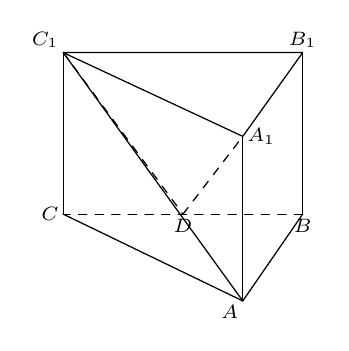
\begin{tikzpicture}[
  x=0.76cm,y=0.76cm,line width=0.45pt,line cap=round,line join=round,
  every node/.style={font=\scriptsize,inner sep=1.5pt}
]
  \coordinate (C)  at (0,1.45);
  \coordinate (B)  at (4.0,1.45);
  \coordinate (D)  at (2.0,1.45);
  \coordinate (A)  at (3.0,0);
  \coordinate (C1) at (0,4.15);
  \coordinate (B1) at (4.0,4.15);
  \coordinate (A1) at (3.0,2.75);

  % Prism edges; BC and the source-indicated interior lines use dashed strokes.
  \draw (C)--(A)--(B);
  \draw[dashed] (B)--(C);
  \draw (C1)--(B1)--(A1)--cycle;
  \draw (C)--(C1) (B)--(B1) (A)--(A1);
  \draw (C1)--(A);
  \draw[dashed] (C1)--(D) (D)--(A1);

  \node[below left] at (A) {$A$};
  \node[below] at (B) {$B$};
  \node[left] at (C) {$C$};
  \node[below] at (D) {$D$};
  \node[right] at (A1) {$A_1$};
  \node[above] at (B1) {$B_1$};
  \node[above left] at (C1) {$C_1$};
\end{tikzpicture}
